%%% Template originaly created by Karol Kozioł (mail@karol-koziol.net) and modified for ShareLaTeX use

\documentclass[a4paper,fleqn,11pt]{article}

\usepackage[T1]{fontenc}
\usepackage[utf8]{inputenc}
\usepackage{graphicx}
\usepackage{xcolor}

\usepackage{tgtermes}

\usepackage[
pdftitle={EE698G - Probabilistic Mobile Robotics Assignment}, 
pdfauthor={Satya Prakash Panuganti, 14610},
colorlinks=true,linkcolor=blue,urlcolor=blue,citecolor=blue,bookmarks=true,
bookmarksopenlevel=2]{hyperref}
\usepackage{amsmath,amssymb,amsthm,textcomp}
\usepackage{enumerate}
\usepackage{multicol}
\usepackage{tikz}

\usepackage{geometry}
\geometry{total={210mm,297mm},
left=25mm,right=25mm,%
bindingoffset=0mm, top=20mm,bottom=20mm}

\usepackage{ mathrsfs }

\linespread{1.3}

\newcommand{\linia}{\rule{\linewidth}{0.5pt}}

% custom theorems if needed
\newtheoremstyle{mytheor}
    {1ex}{1ex}{\normalfont}{0pt}{\scshape}{.}{1ex}
    {{\thmname{#1 }}{\thmnumber{#2}}{\thmnote{ (#3)}}}

\theoremstyle{mytheor}
\newtheorem{defi}{Definition}

% my own titles
\makeatletter
\renewcommand{\maketitle}{
\begin{center}
\vspace{2ex}
{\huge \textsc{\@title}}
\vspace{1ex}
\\
\linia\\
\@author \hfill \@date
\vspace{4ex}
\end{center}
}
\makeatother
%%%

% custom footers and headers
\usepackage{fancyhdr,lastpage}
\pagestyle{fancy}
\lhead{}
\chead{}
\rhead{}
\lfoot{Assignment 1}
\cfoot{}
\rfoot{Page \thepage\ /\ \pageref*{LastPage}}
\renewcommand{\headrulewidth}{0pt}
\renewcommand{\footrulewidth}{0pt}
%

%%%----------%%%----------%%%----------%%%----------%%%

\begin{document}

\title{EE698G - Probabilistic Mobile Robotics Assignment}

\author{Satya Prakash Panuganti, 14610}

\date{22 January, 2017}

\maketitle

\section{}
$<p_{i}, p_{j}>$ $= 0$ $\forall$ $i \neq j$ $\&$ $1 \leqslant i, j \leqslant n$ and $p_{i} \neq 0$ $\forall$ $1 \leqslant i \leqslant n$ \\
Let us assume that $\{p_{1}, p_{2}, ... , p_{n}\}$ is linearly dependent. \\
$\therefore$ \hspace{2ex}$ \sum_{i=1}^{n} c_{i}p_{i} = 0$ $\&$ $\{c_{1}, c_{2}, ... , c_{n}\} \neq \{0, 0, ... , 0\}.$ \\
$\implies c_{j} \neq 0$ for some $j$ such that $1 \leqslant j \leqslant n.$ \\
$\implies c_{j}p_{j} = - \sum_{i \neq j, 1 \leqslant i \leqslant n} c_{i}p_{i}$ \\
$\implies <p_{j}, c_{j}p_{j}>$ $=$ $<p_{j}, - \sum_{i \neq j, 1 \leqslant i \leqslant n} c_{i}p_{i}>$ \\
$\implies c_{j}<p_{j}, p_{j}>$ $= - \sum_{i \neq j, 1 \leqslant i \leqslant n} c_{i}<p_{j}, p_{i}>$
\begin{equation}
\implies c_{j}<p_{j}, p_{j}> \hspace{1ex} = 0
\end{equation}
Now, $p_{i} \neq 0$ $\forall$ $1 \leqslant i \leqslant n$ \\
$\therefore$ $<p_{j}, p_{j}>$ $= k \neq 0$ where $k \in \!R.$ \\
Also, $c_{j} \neq 0$ 
\begin{equation}
\implies c_{j}<p_{j}, p_{j}> \hspace{1ex} \neq 0.
\end{equation}
$\therefore$ We have a contradiction from (1) \& (2).\\
Hence, $\{p_{1}, p_{2}, ... , p_{n}\}$ is linearly independent.

\section{}
Let $H = \begin{bmatrix}
		 H_{A} \\
		 H_{B} \\
		 H_{C}
		 \end{bmatrix}$ be the real heights and $\hat{H} = \begin{bmatrix}
															 \hat{H_{A}} \\
															 \hat{H_{B}} \\
															 \hat{H_{C}}
															 \end{bmatrix}$
be the estimated heights of the buildings A, B \& C. \\ \\
Expressing the the data collected by the sensor in the form $A\hat{H} + e = b$, where e is the error vector, we have : \\ \\
Now, $\begin{bmatrix}
	  1  & -1 & 0  \\
	  1  & 0  & -1 \\
	  0  & 1  & -1 \\
	  1  & 0  & 0  \\
	  0  & 1  & 0  \\
	  0  & 0  & 1  \\
	  \end{bmatrix}
	  \begin{bmatrix}
	  \hat{H_{A}} \\
	  \hat{H_{B}} \\
	  \hat{H_{C}}
	  \end{bmatrix} + e
	  =
	  \begin{bmatrix}
	  -14.22 \\
	  -23.55 \\
	  -9.5   \\
	  24.64  \\
	  38.8   \\
	  48.3
	  \end{bmatrix}$ using the data provided by the instrument. \\ \\

On minimizing LSE, we have $\hat{H} = (A^T A)^{-1} A^T b = \begin{bmatrix}
															 24.65 \\
															 38.82 \\
															 48.27
															 \end{bmatrix}$ \begin{flushright}
[Solved using GNU Octave 4.0.0; File : `/code/question2.m']
\end{flushright}

\section{}

The $\mathscr{L}agrangian$ is given by: \\
$\mathscr{L} = x^T Q x - \lambda (x^T x - I)$ \& $\lambda \neq 0.$ \\
Maximizing $x^T Qx$, we have : 
$\frac{\partial \mathscr{L}}{\partial x} = 0$ \\
$\implies Qx = \lambda x$ \\
$\implies (Q - \lambda I)x = 0$ \\
$\implies \|Q - \lambda I\| = 0$ \\
Also,
\begin{equation}
x^T Qx = x^T \lambda x = \lambda x^T x = \lambda
\end{equation}

Hence, x is the eigenvector corresponding to the maximum eigenvalue of Q. \\
The eigenvalues of Q are $1 \pm 0.5$. \\
Choosing $\lambda$ as $1.5$, we get $Qx = \lambda x$ \\ \\
Taking $x = \begin{bmatrix}
			x_{1} \\
			x_{2}
			\end{bmatrix}$, \hspace{1ex}
$Q \begin{bmatrix}
   x_{1} \\
   x_{2}
   \end{bmatrix} = 1.5x$, we have : \\ \\
$x_{1} + 0.5x_{2} = 1.5x_{1} \implies x_{1} = x_{2}$ \& $0.5x_{1} + x_{2} = 1.5x_{2} \implies x_{1} = x_{2}$ \\ \\
Ensuring $\|x\| = 1 \implies x = \begin{bmatrix}
								  \frac{1}{\sqrt{2}} \\
								  \frac{1}{\sqrt{2}}
								  \end{bmatrix} or
								  \begin{bmatrix}
								  -\frac{1}{\sqrt{2}} \\
								  -\frac{1}{\sqrt{2}}
								  \end{bmatrix}$
are values of x for which the maximum value of $x^T Q x$ occurs for $\|x\| = 1$. \\
The maximum value of  $x^T Q x$ is 1.5 [from (3)].
\section{}
\subsection{(a)}
\subsubsection*{(i)}
We have, $e^{x^2} > 0$ $\forall$ $x$ as $e^{-t} > 0$ $\forall \in \!R$. \\
Also, $\sigma > 0 \implies \frac{1}{\sigma \sqrt{2} \pi} > 0$ \\
$\implies f_{X}(x) = \frac{1}{\sigma \sqrt{2\pi}} e^{\frac{-(x - \mu)^2}{2 \sigma^2}} > 0$ $\forall$ $x \in \!R$
\subsubsection*{(ii)}
$f_{X}$ is also clearly continuous.
\subsubsection*{(iii)}
\begin{align*}
Let \hspace{1ex} & J = \int_{-\infty}^{\infty} f_{X} dx. \\
& = \int_{-\infty}^{\infty} \frac{1}{\sigma \sqrt{2\pi}} e^{\frac{-(x - \mu)^2}{2 \sigma^2}} dx. \\
Let \hspace{1ex} & t = \frac{x - \mu}{\sqrt{2} \sigma}. \\
\implies & dx = \sqrt{2} \sigma dt \\
\implies & J = \frac{1}{\sqrt{\pi}}\int_{-\infty}^{\infty} e^{-t^2} dt \\
Let \hspace{1ex} & I = \int_{-\infty}^{\infty} e^{-t^2} dt \\
\implies & I^2 = \int_{-\infty}^{\infty} e^{-t_{1}^2} dt_{1} \int_{-\infty}^{\infty} e^{-t_{2}^2} dt_{2} \\
\implies & \hspace{2ex} = \int_{-\infty}^{\infty}\int_{-\infty}^{\infty} e^{-(t_{1}^2 + t_{2}^2)} dt_{1} dt_{2} \\
Taking \hspace{1ex} t_{1}^2 + t_{2}^2 = r^2, \\
dt_{1}dt_{2} = rd \theta dr \\
\implies & I^2 = \int_{0}^{2\pi}(\int_{-\infty}^{\infty} r e^{-r^2} dr) d \theta \\
Let \hspace{1ex} r^2 = \lambda \\
\implies 2r dr = d\lambda \implies r dr = \frac{d\lambda}{2} \\
\implies & I^2 = \frac{1}{2} \int_{0}^{2\pi}(\int_{0}^{\infty} e^\lambda d\lambda) d \theta \\
& \hspace{2ex} = \pi \\
\implies & I = \sqrt{\pi} \\
\implies & J = \frac{1}{\sqrt{\pi}} \sqrt{\pi} \\
\implies & \int_{-\infty}^{\infty} f_{X} dx = 1
\end{align*}
(i), (ii) \& (iii) $\implies f_{X}$ is a valid p.d.f.
\subsection{(b)}
$f_{X} (\mu + x) = \frac{1}{\sigma \sqrt{2\pi}} e^{-\frac{x^2}{2\sigma^2}}$ \\
$f_{X} (\mu - x) = \frac{1}{\sigma \sqrt{2\pi}} e^{-\frac{x^2}{2\sigma^2}}$ \\
Hence, $f_{X} (\mu + x) = f_{X} (\mu - x)$ \\
$\therefore f_{X}$ is symmetric about $\mu$. \\
\subsection{(c)}
\begin{align*}
mean, \hspace{1ex} & E[X] = \int_{-\infty}^{\infty} x f_{X} (x) dx \\
& \hspace{5ex} = \int_{-\infty}^{\infty} x \frac{1}{\sigma \sqrt{2\pi}} e^{\frac{-(x - \mu)^2}{2 \sigma^2}} dx \\
Let \hspace{1ex} t = \frac{x - \mu}{\sqrt{2} \sigma}. \\
\implies x = \sqrt{2} \sigma t + \mu \\
\implies dx = \sqrt{2} \sigma dt \\
\therefore \hspace{1ex} & E[X] = \int_{-\infty}^{\infty} \frac{1}{\sigma \sqrt{2\pi}} (\sqrt{2}\sigma t + \mu) e^{-t^2} dt \\
& \hspace{5ex} = \int_{-\infty}^{\infty} \frac{t e^{-t^2}}{\sqrt{\pi}} dt + \int_{-\infty}^{\infty} \frac{\mu e^{-t^2}}{\sqrt{\pi}} dt \\
Now, \hspace{1ex} & \int_{-\infty}^{\infty} \frac{t e^{-t^2}}{\sqrt{\pi}} dt = 0 &\because \hspace{1ex} it \hspace{1ex} is \hspace{1ex} an \hspace{1ex} odd \hspace{1ex} function \\
\& \hspace{1ex} & \int_{-\infty}^{\infty} \frac{\mu e^{-t^2}}{\sqrt{\pi}} = \mu & [Using \hspace{1ex} result \hspace{1ex} of \hspace{1ex} 4.1(a)(iii)] \\
\therefore \hspace{1ex} & mean, \hspace{1ex} \hspace{1ex} E[X] = \mu
\end{align*}
\begin{align*}
variance, \hspace{1ex} & \Sigma_{X} = E[X^2] - E[X]^2 \\
& E[X^2] = \int_{-\infty}^{\infty} x^2 f_{X} dx \\
& \hspace{6ex} = \int_{-\infty}^{\infty} \frac{1}{\sigma\sqrt{2\pi}} x^2 e^{-(\frac{(x - \mu)^2}{2\sigma^2})} dx \\
Let \hspace{1ex} t = \frac{x - \mu}{\sqrt{2} \sigma}. \\
\implies x = \sqrt{2} \sigma t + \mu \\
\implies dx = \sqrt{2} \sigma dt \\
\therefore \hspace{1ex} & E[X^2] = \int_{-\infty}^{\infty} \frac{(\sqrt{2}\sigma t + \mu)^2}{\sqrt{\pi}} e^{-t^2} dt \\
& \hspace{6ex} = \int_{-\infty}^{\infty} \frac{2\sigma^2 t^2}{\sqrt{\pi}} e^{-t^2} dt +  \int_{-\infty}^{\infty} \frac{\mu^2}{\sqrt{\pi}} e^{-t^2} dt + \int_{-\infty}^{\infty} \frac{2\sqrt{2}\sigma t}{\sqrt{\pi}} e^{-t^2} dt \\
Now, \hspace{1ex} & \int_{-\infty}^{\infty} \frac{2\sqrt{2}\sigma t}{\sqrt{\pi}} e^{-t^2} dt = 0 \hspace{18ex} \because  \hspace{1ex} it \hspace{1ex} is \hspace{1ex} an \hspace{1ex} odd \hspace{1ex} function \\
\& \hspace{1ex} & \int_{-\infty}^{\infty} \frac{\mu^2}{\sqrt{\pi}} e^{-t^2} = \mu^2 \hspace{20ex} [Using \hspace{1ex} result \hspace{1ex} of \hspace{1ex} 4.1(a)(iii)] \\
\therefore \hspace{1ex} & E[X^2] = \int_{-\infty}^{\infty} \frac{2\sigma^2 t^2}{\sqrt{\pi}} e^{-t^2} dt +  \mu^2 \\
Let \hspace{1ex} I = \int_{-\infty}^{\infty} t^2 e^{-t^2} dt \\
\implies I^2 & = \int_{-\infty}^{\infty} t_{1}^2 e^{-t_{1}^2} dt_{1} \int_{-\infty}^{\infty} t_{2}^2 e^{-t_{2}^2} dt_{2} \\
& = \int_{-\infty}^{\infty} t_{1}^2 t_{2}^2 e^{-t_{1}^2} e^{-t_{2}^2} dt_{1} dt_{2} \\
Taking \hspace{1ex} t_{1}^2 + t_{2}^2 = r^2, \\
dt_{1}dt_{2} = rd \theta dr \\
\implies I^2 & = \int_{0}^{2\pi} (\int_{0}^{\infty} r^5 e^{-r^2} dr) sin^4 \theta cos^4 \theta d\theta \\
Let \hspace{1ex} & J = \int_{0}^{\infty} r^5 e^{-r^2} dr \hspace{1ex} \& \hspace{1ex} K = \int_{0}^{2\pi} sin^4 \theta cos^4 \theta d\theta \\
Let \hspace{1ex} r^2 = \lambda \\
\implies 2r dr = d\lambda \implies r dr = \frac{d\lambda}{2} \\
\implies J & = \frac{1}{2} \int_{0}^{\infty} t^2 e^{-t} dt \\
& = \frac{1}{2} \int_{0}^{\infty} 2t e^{-t} dt \hspace{6ex} [By \hspace{1ex} using \hspace{1ex} Integration \hspace{1ex} by \hspace{1ex} parts] \\
& = \frac{2}{2} \int_{0}^{\infty} e^{-t} dt = 1 \hspace{4ex} [By \hspace{1ex} using \hspace{1ex} Integration \hspace{1ex} by \hspace{1ex} parts \hspace{1ex}
 again] \\ 
Now, \hspace{1ex} K & = \int_{0}^{2\pi} sin^4 \theta cos^4 \theta d\theta \\
& = \frac{1}{4} \int_{0}^{2\pi} sin^2 (2\theta) d\theta \\
& = \frac{1}{4} \int_{0}^{2\pi} \frac{1 - cos (4\theta)}{2} d\theta \\
& = \frac{\pi}{4} \\
\end{align*}
\begin{align*}
Now, \hspace{1ex} I^2 & = J K \\
& = \frac{\pi}{4} \\
\implies I & = \frac{\sqrt{\pi}}{2} \\
\therefore \hspace{1ex} & E[X^2] = \frac{2\sigma^2}{\sqrt{\pi}} I + \mu^2 \\
& \hspace{6ex} = \frac{2\sigma^2}{\sqrt{\pi}}\frac{\sqrt{\pi}}{2} + \mu^2  \\
& \hspace{6ex} = \sigma^2 + \mu^2 \\
Hence, \hspace{1ex} variance, \hspace{1ex} & \Sigma_{X} = E[X^2] - E[X]^2 \\
& \hspace{3ex} = \sigma^2 + \mu^2 - \mu^2 \\
& \hspace{3ex} = \sigma^2
\end{align*}
\section{}
We know that :
\begin{center}
If $g : S_X$ → $\!R$ is strictly monotone with inverse function $g^{-1} (y)$ such that $\frac{dg^{-1} (y)}{dy}$ is continuous. Let
$g(S_X) = \{g (x)\ :\ x\ \in\ S_X\}$. Then, $Y = g (X)$ is an absolutely continuous random variable with p.d.f : \\
$f_Y (y) = f_X (g^{-1}(y)) | \frac{dg^{-1}(y)}{dy} | I_{g(S_X)} (y)$ \\
where, for a set A, $I_A ($·$)$ denotes its indicator function, i.e.,
$I_A = \begin{cases}
		1,\ if\ y\ \in\ A \\
		0,\ otherwise
		\end{cases}$
\end{center}
Also, $\because$ X and Y have uniform distribution U[0, 1], $f_{X}(x) = f_{Y}(y) = 1$ for $x$ $\in$ [0, 1] and  for $y$ $\in$ [0, 1] respectively. Both $f_{X}(x)\ \&\ f_{Y}(y)$ are equal to 0 outside of [0, 1].
\subsection*{(a)}
$Z_{1} := log(\frac{1}{X})$ \\
Let $g_{1}(x) = log(\frac{1}{x})$ \\
Now, $g_{1}$ is both continuous and strictly monotonous for [0, 1]
\begin{align*}
Also, \hspace{1ex} & z_{1}(x) = g_{1}(x) \hspace{1ex} & for \hspace{1ex} x \in [0, \hspace{1ex} 1] \\
Clearly, \hspace{1ex} & z_{1}(x) = g_{1}(x) \in [0, \hspace{1ex} \infty) \hspace{1ex} & for \hspace{1ex} x \in [0, \hspace{1ex} 1] \\
\therefore \hspace{1ex} & f_{Z_{1}}(z_{1}) = f_{X} (x) |(\frac{dg_{1} (x)}{dx})^{-1}|\ & for \hspace{1ex} x \in [0, \hspace{1ex} 1] \\
& \hspace{7ex} = x\ & for \hspace{1ex} x \in [0, \hspace{1ex} 1] \\
Now, \hspace{1ex} & z_{1} = log (\frac{1}{x}) \\
\implies \hspace{1ex} & \frac{1}{x} = e^{z_{1}} \\
\implies \hspace{1ex} & x = e^{-z_{1}} \\
Hence, \hspace{1ex} & f_{Z_{1}}(z_{1}) = e^{-z_{1}} \hspace{1ex} & for \hspace{1ex} z_{1} \in [0,\infty) \\
Also, \hspace{1ex} & f_{Z_{1}}(z_{1}) = 0 \hspace{1ex} & if \hspace{1ex} z_{1} < 0
\end{align*}
\subsection*{(b)}
$Z_{2} := e^X$ \\
Let $g_{2}(x) = e^x$ \\
Now, $g_{2}$ is both continuous and strictly monotonous for [0, 1].
\begin{align*}
Also, \hspace{1ex} & z_{2}(x) = g_{2}(x) \hspace{1ex} & for \hspace{1ex} x \in [0, \hspace{1ex} 1] \\
Clearly, \hspace{1ex} & z_{2}(x) = g_{2}(x) \in [1, \hspace{1ex} e] \hspace{1ex} & for \hspace{1ex} x \in [0, \hspace{1ex} 1] \\
\therefore \hspace{1ex} & f_{Z_{2}}(z_{2}) = f_{X} (x) |(\frac{dg_{2} (x)}{dx})^{-1}| \hspace{1ex} & for \hspace{1ex} x \in [0, \hspace{1ex} 1] \\
& \hspace{7ex} = e^x \hspace{1ex} & for \hspace{1ex} x \in [0, \hspace{1ex} 1] \\
Now, \hspace{1ex} & z_{2} = e^{-x} \\
\implies \hspace{1ex} & x = log (z_{2}) \\
Hence, \hspace{1ex} & f_{Z_{2}}(z_{2}) = e^{-log (z_{2})} \hspace{1ex} & for \hspace{1ex} x \in [0, \hspace{1ex} 1]  \\
& \hspace{7ex} = \frac{1}{z_{2}} \hspace{1ex} & for \hspace{1ex} z_{2} \in [1, \hspace{1ex} e) \\
Also, \hspace{1ex} & f_{Z_{2}}(z_{2}) = 0 \hspace{1ex} & if \hspace{1ex} z_2 \not\in [1, \hspace{1ex} e)
\end{align*}
\subsection*{(c)}
Let $F_{Z_3}$ be the distribution function of $Z_{3}$
\begin{align*}
joint \hspace{1ex} p.d.f \hspace{1ex} of \hspace{1ex} X, \hspace{1ex}Y; \hspace{1ex} f_{X,Y}(x,y) & = f_{X}(x)f_{Y}(y) & \because \hspace{1ex} X, \hspace{1ex} Y \hspace{1ex} are \hspace{1ex} i.i.d \\
& = \begin{cases}
	1 \hspace{1ex} if \hspace{1ex} 0 \leq x,y \leq 1 \\
	0 \hspace{1ex} otherwise \\
	\end{cases} \\
Also, \hspace{1ex} F_{Z_3}(z) & = \int_{-\infty}^{z - t_{1}} (\int_{-\infty}^{\infty} f_{X,Y}(t_{1},t_{2}) dt_{1}) dt_{2} \\
F_{Z_3}(z) & = 0 \hspace{1ex} & if \hspace{1ex} z \leq 0 \\
We \hspace{1ex} have, \hspace{1ex} F_{Z_3}(z) & =  \int_{0}^{z} (\int_{0}^{z - t_{1}} 1 \hspace{1ex} dt_{2}) dt_{1} \hspace{1ex} & if \hspace{1ex} 0 \hspace{1ex} < z \leq 1 \\
& = \int_{0}^{z} (z - t_{1}) dt_{1} \hspace{1ex} & if \hspace{1ex} 0 \hspace{1ex} < z \leq 1 \\
& = \frac{z^2 }{2} \hspace{1ex} & if \hspace{1ex} 0 \hspace{1ex} < z \leq 1 \\
Now, \hspace{1ex} P (\{ Z_3 > z\}) & = \int_{z-1}^{1} (\int_{z - t_{1}}^{1} 1 \hspace{1ex} dt_{2}) dt_{1} \hspace{1ex} & if \hspace{1ex} 1 \hspace{1ex} < z \leq 2 \\
& = \int_{z - 1}^{1} (1 - z + t_{1}) dt_{1} \hspace{1ex} & if \hspace{1ex} 1 \hspace{1ex} < z \leq 2 \\
& = (2 - z)(1 - z) + \frac{1 - (z-1)^2}{2} \hspace{1ex} & if \hspace{1ex} 1 \hspace{1ex} < z \leq 2 \\
& = 2 - 3z + z^2 + \frac{2z - z^2}{2} \hspace{1ex} & if \hspace{1ex} 1 \hspace{1ex} < z \leq 2 \\
& = 2 - 2z + \frac{z^2}{2} \hspace{1ex} & if \hspace{1ex} 1 \hspace{1ex} < z \leq 2 \\
We \hspace{1ex} know \hspace{1ex} that, \hspace{1ex} F_{Z_3}(z) & = 1 - P (\{ Z > z\}) \\
& = 1 - (2 - 2z + \frac{z^2}{2}) \hspace{1ex} & if \hspace{1ex} 1 \hspace{1ex} < z \leq 2 \\
& = -1 + 2z - \frac{z^2}{2} \hspace{1ex} & if \hspace{1ex} 1 \hspace{1ex} < z \leq 2 \\
Also, \hspace{1ex} F_{Z_3}(z) & = 1 \hspace{1ex} & if \hspace{1ex} z \geq 2 \\
\because \hspace{1ex} p.d.f \hspace{1ex} of \hspace{1ex} Z_3, \hspace{1ex} f_{Z_3}(z) & = \frac{dF_{Z_3}(z)}{dz}, \hspace{1ex} we \hspace{1ex} have : \\
f_{Z_3}(z) & = \begin{cases}
					z \hspace{1ex} & if \hspace{1ex} 0 \hspace{1ex} < z \leq 1 \\
					2 - z \hspace{1ex} & if \hspace{1ex} 1 \hspace{1ex} < z \leq 2 \\
					0 \hspace{1ex} & otherwise
				\end{cases}
\end{align*}
\section{}
\subsection*{(a)}
$\because\ P (B \cap C) > 0,\ P (B) > 0\ \&\ P (C) > 0$
\begin{align*}
Now, \hspace{1ex} P (A \cap B | C) & = \frac{P(A \cap B \cap C)}{P(C)} \\
P(A | B \cap C) & = \frac{P(A \cap B \cap C)}{P(B \cap C)} \\
\&\ P(B | C) & = \frac{P(B \cap C)}{P(C)} \\
\therefore\ P(A | B \cap C)P(B | C) & = \frac{P(A \cap B \cap C)}{P(C)}
\end{align*}
Hence, proved.
\subsection*{(b)}
Let $\varepsilon$ be the random experiment of the casting of a red die and green die. \\
Let $A$ be the event that an even number appears on the red die, \\
$B$ be the event that an odd number appears on the green die, \\
and $C$ be the event that sum of the numbers on the dice is 7. \\
Clearly, events $A$ and $B$ are independent events. \\
Using relative frequency model for assigning probability,
\begin{align*}
P (A \cap B | C) = \frac{3}{6} = 0.5 \hspace{2ex} & [even \hspace{1ex} number \hspace{1ex}appears \hspace{1ex} on \hspace{1ex} red \hspace{1ex} die \\
& and\ odd \hspace{1ex} number \hspace{1ex} appears \hspace{1ex} on \hspace{1ex} green \hspace{1ex} die, \\
& given \hspace{1ex} that \hspace{1ex} the \hspace{1ex} sum \hspace{1ex} is \hspace{1ex} 7]\\
P (A | C) = \frac{3}{6} = 0.5 \hspace{2ex} & [even \hspace{1ex} number \hspace{1ex}appears \hspace{1ex} on \hspace{1ex} red \hspace{1ex} die \\
& given \hspace{1ex} that \hspace{1ex} the \hspace{1ex} sum \hspace{1ex} is \hspace{1ex} 7]\\
P (B | C) = \frac{3}{6} = 0.5 \hspace{2ex} & [odd \hspace{1ex} number \hspace{1ex}appears \hspace{1ex} on \hspace{1ex} green \hspace{1ex} die \\
& given \hspace{1ex} that \hspace{1ex} the \hspace{1ex} sum \hspace{1ex} is \hspace{1ex} 7]\\
\therefore \hspace{1ex} P (A | C) P (B | C) = 0.5^2 = 0.25
\end{align*}
$But, \hspace{1ex} P (A \cap B | C) = 0.5 \neq P (A | C) P (B | C) = 0.25$ \\
Hence, the premise that $P (A \cap B | C) = P (A | C) P (B | C)$ if A and B are independent events is false.
\pagebreak
\section{}
We are given $X =\{\vec{x_{1}},\vec{x_{2}},...,\vec{x_{n}}\}$, $\vec{x_{i}} \in \!R^d$ $\forall$ $1 \leq i \leq n$ \\
Let $\vec{a} \in \!R^d$ such that $\|\vec{a}\| = 1$ and variance of $P = \{p_{1},p_{2},\hdots,p_{n}\}$ is maximum, where $p_{i}$ is the projection of $\vec{x_{i}}$ along $\vec{a}$. \\
Now, variance of $P$, V  = $\frac{1}{n}\sum_{i = 1}^{n} \|p_{i} - \bar{p}\|^2$, where $\bar{p}$ is the mean of P.
\begin{align*}
p_{i} & = \vec{a}^T\vec{x_{i}} \\
\implies \bar{p} & = \frac{1}{n}\sum_{1}^{n} p_{i} \\
& = \frac{1}{n}\sum_{1}^{n} \vec{a}^T\vec{x_{i}} \\
& = \vec{a}^T\frac{1}{n}\sum_{1}^{n} \vec{x_{i}} \\
& = \vec{a}^T \vec{\mu}_{X} \hspace{1ex} where \hspace{1ex} \vec{\mu}_{X} \hspace{1ex} is \hspace{1ex} the \hspace{1ex} mean \hspace{1ex} of \hspace{1ex} X\\
Also, \hspace{1ex} V & = \frac{1}{n}\sum_{i = 1}^{n} \|p_{i} - \bar{p}\|^2 \\
& = \frac{1}{n}\sum_{i = 1}^{n} (\vec{a}^T\vec{x_{i}} - \bar{p})^2 \\
& = \frac{1}{n}\sum_{i = 1}^{n} (\vec{a}^T\vec{x_{i}} - \vec{a}^T \vec{\mu}_{X})^2 \\
& = \frac{1}{n}\sum_{i = 1}^{n} (\vec{a}^T(\vec{x_{i}} - \vec{\mu}_{X}))^2 \\
& = \frac{1}{n}\sum_{i = 1}^{n} (\vec{a}^T(\vec{x_{i}} - \vec{\mu}_{X}))(\vec{a}^T(\vec{x_{i}} - \vec{\mu}_{X}))^T \\
& = \frac{1}{n}\sum_{i = 1}^{n} \vec{a}^T(\vec{x_{i}} - \vec{\mu}_{X})(\vec{x_{i}} - \vec{\mu}_{X})^T\vec{a} \\
& = \frac{1}{n}\sum_{i = 1}^{n} \vec{a}^T(\vec{x_{i}} - \vec{\mu}_{X})(\vec{x_{i}} - \vec{\mu}_{X})^T\vec{a} \\
& = \vec{a}^T(\frac{1}{n}\sum_{i = 1}^{n}(\vec{x_{i}} - \vec{\mu}_{X})(\vec{x_{i}} - \vec{\mu}_{X})^T)\vec{a} \\
& = \vec{a}^T Q\vec{a}, \hspace{1ex} where \hspace{1ex} Q \hspace{1ex} is \hspace{1ex} the \hspace{1ex} covariance \hspace{1ex} matrix \hspace{1ex} of \hspace{1ex} X.
\end{align*}
As $\|\vec{a}\| = 1$, the $\mathscr{L}agrangian$ is given by: \\
$\mathscr{L} = \vec{a}^T Q \vec{a} - \lambda (\vec{a}^T \vec{a} - I)$ \& $\lambda \neq 0.$ \\
Maximizing $\vec{a}^T Q \vec{a}$, we have : 
$\frac{\partial \mathscr{L}}{\partial \vec{a}} = 0$ \\
$\implies Q\vec{a} = \lambda \vec{a}$ \\
$\implies (Q - \lambda I)\vec{a} = 0$ \\
$\implies \|Q - \lambda I\| = 0$ \\
Also,
\begin{equation*}
\vec{a}^T Q\vec{a} = \vec{a}^T \lambda \vec{a} = \lambda \vec{a}^T \vec{a} = \lambda
\end{equation*}
Hence, $\vec{a}$ is the eigenvector corresponding to the maximum eigenvalue of Q which is the sample covariance matrix. \\
$\therefore$ The direction of maximum variance is given by the eigenvector corresponding to the maximum eigenvalue of the sample covariance matrix of the data. \\
Hence, proved. \\
$\because Q = (\frac{1}{n}\sum_{i = 1}^{n}(\vec{x_{i}} - \vec{\mu}_{X})(\vec{x_{i}} - \vec{\mu}_{X})^T)$, it is a $d \times d$ matrix as $x_{i}$ \& $\vec{\mu}_{X}$ are $d$ dimensional vectors. \\
The number of principal components can be taken as n where $1 \leq n \leq d,$ $n \in \!N$.
\section{}
\subsection{(a)}
\begin{center}
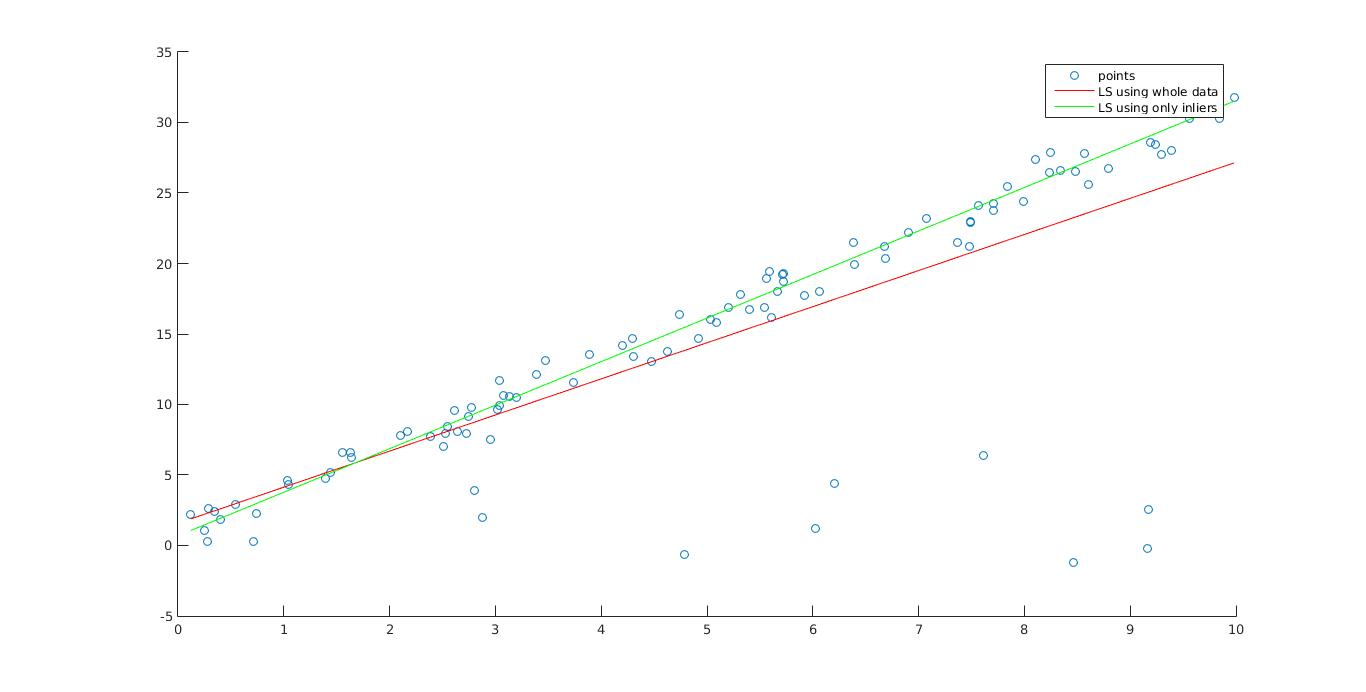
\includegraphics[scale = 0.35]{../images/ols.jpg}
\end{center}
The line obtained through LSE after running RANSAC algorithm to obtain the inliers set is better than the the line obtained by simply applying LSE over the test data; since on observation, the RANSAC line is closer to more points than the basic line estimate is.
\pagebreak
\subsection{(b)}
\begin{center}
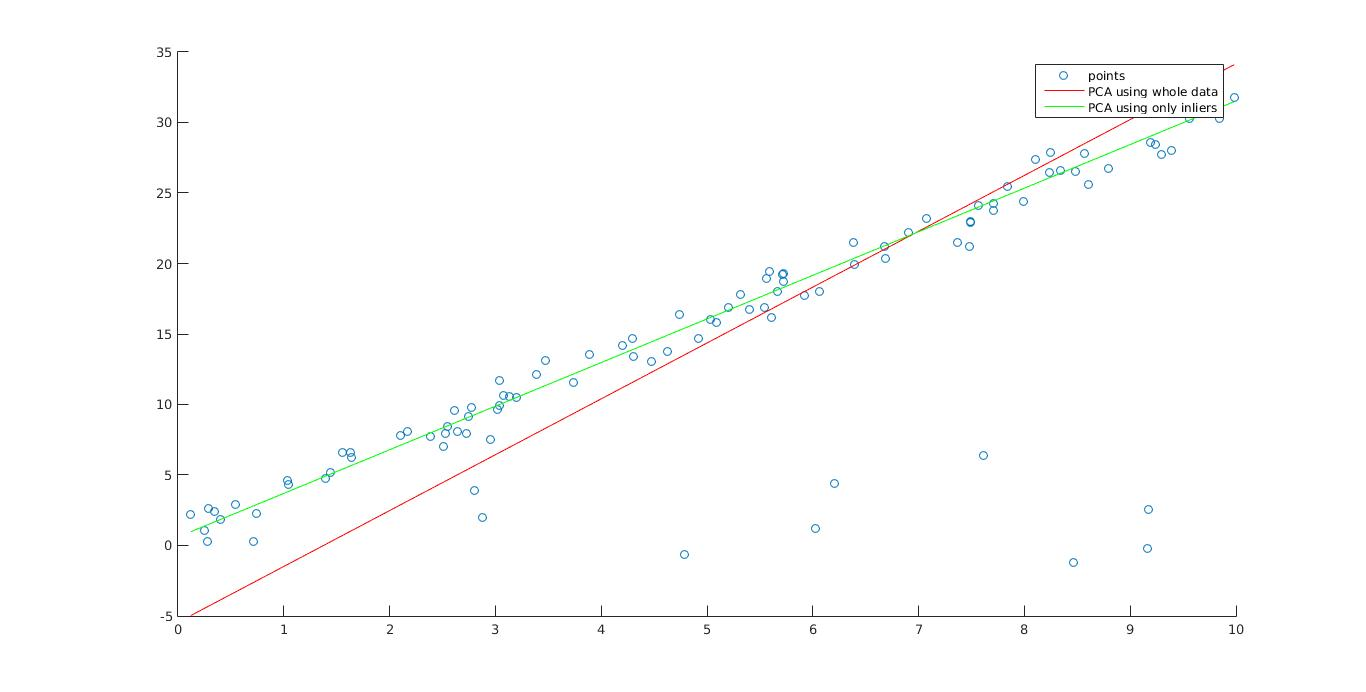
\includegraphics[scale = 0.35]{../images/pca.jpg}
\end{center}
The line obtained through PCA after running RANSAC algorithm to obtain the inliers set is better than the the line obtained by simply applying PCA over the test data; since on observation, the RANSAC line is closer to more points than the basic line estimate is.
\subsection*{Remark:}
From the above two experiments, it can be inferred that applying RANSAC algorithm over sample data to remove outliers is an effective way to reduce skew in estimates stemming from extreme errors.
\section{}
\begin{center}
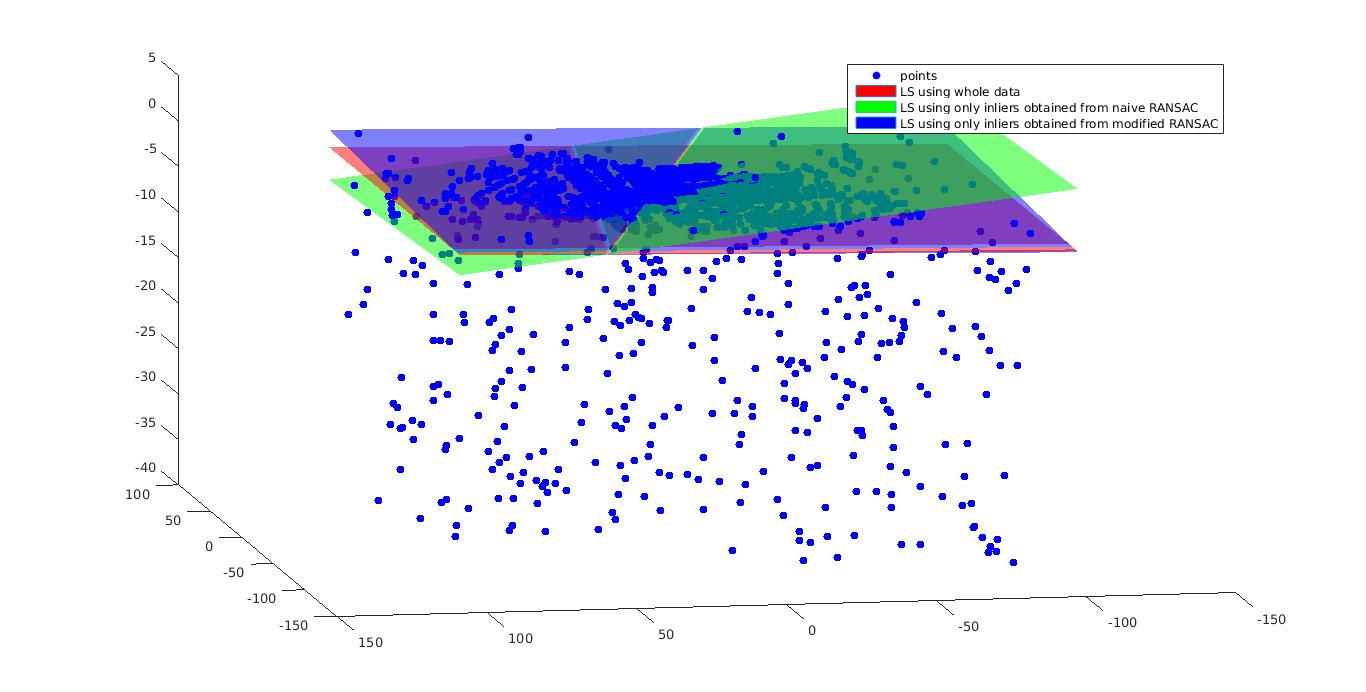
\includegraphics[scale = 0.35]{../images/q9.jpg}
\end{center}
I implemented two versions of RANSAC :
\subsection*{(i) Naive Method}
In this method, only 3 points are chosen during the trial stage of the RANSAC algorithm. On using this implementation, highly skewed planes were often appearing even on setting the `inlier set probability' parameter to 0.99. This artifact can be attributed to large variations among the inlier points along the direction perpendicular to the actual plane.
\subsection*{(ii) Modified Method}
To account for the problem described above, a modified RANSAC implementation was developed, in which, `s' (= 25) points are taken while fitting a model during a trial. I observed that on choosing 25 points, the implementation regularly generates a plane which on observation appears to be a good fit for the provided data points in a reasonable amount of time.
\end{document}